\documentclass{article}

% Lenguaje y Fuente
\usepackage[spanish]{babel}
\usepackage[utf8x]{inputenc}
\usepackage[T1]{fontenc}
\usepackage[top=1in, bottom=1.25in, left=1.1 in, right=1.1 in]{geometry}
\usepackage{graphicx}

% Portada

\title{\textbf{Reporte de la Actividad 1}\\ Aumento de la Temperatura Global}
\author{Luis Fernando Duarte Gonzalí \\ Universidad de Sonora \\ Física Computacional}
\date{Enero del 2019}
\begin{document}
\maketitle

% Contenido del Reporte

\section{Introducción}
El siguiente reporte formará parte de la lista de actividades de la clase de física computacional con el fin de crear un resumen de los aspectos de mi interés en el reporte de 1.5°C del IPCC. Se abordará el tema del aumento de la temperatura global y formas para detenerlo.

\section{Entendiendo $1.5$°C: Niveles de referencia, Probabilidad, Transitoriedad, Rebasamiento y Estabilización.}

\subsection{Definiciones prácticas de $1.5$°C y $2.0$°C}
En el reporte se define el calentamiento como como un incremento en algunas décadas de la temperatura media de la superficie por encima de los niveles pre-industriales. Más específicamente, el calentamiento en un tiempo dado está definido como el promedio global de las temperaturas combinadas de la superficie de tierra, aire y superficie del océano por un periodo de 30 años centrado en ese punto del tiempo dado, expresando el relativo tomando el periodo 1850-1900 como los niveles aproximados del tiempo pre-industrial, pero excluyendo el impacto  natural. 

El reporte de la IPCC toma como una definición práctica del $1.5$°C relativa a los niveles pre-industriales que corresponde al promedio de las temperaturas globales combinadas del aire de la superficie y los océanos ambas 1.5°C más cálido que el promedio del periodo de 51 años 1850-1900, 0.87°C más cálido que en el periodo de 20 años 1986-2005, o 0.63°C más cálido que en la década de 2006-2015.

\subsubsection{Calentamiento total contra calentamiento inducido por el humano y tasas de calentamiento.}

Se refiere al calentamiento total como el cambio actual de la temperatura, sin tomar en cuenta la causa, mientras que el calentamiento inducido por el humano se refiere al componente de ese total atribuido a la actividad humana. Los estudios de mitigación se enfocan en el calentamiento inducido por la actividad humana, mientras que los estudios de los impactos del cambio climático se refieren al calentamiento total.

Cuando se omite la actividad volcánica y los cambios en el sol que afectan a la tierra dentro del calentamiento total, la diferencia entre éstas y por actividad humana es muy pequeña.  En la siguiente figura se puede observar que el nivel del calentamiento inducido por el humano ha sido indistinguible del calentamiento total desde el año 2000 incluyendo la década de 2006-2015.
\begin{figure}[h]
    \centering
    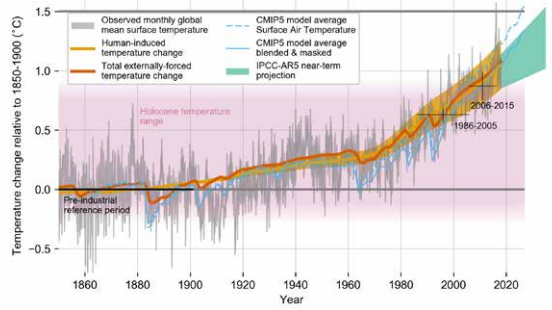
\includegraphics[scale=0.8]{Figura1}
    \caption{Evolución de la temperatura promedio global de la superficie (GMST) sobre el tiempo de observaciones instrumentales.}
    \label{Figura 1}
\end{figure}

Ya que el calentamiento está definido en términos de un promedio de 30 años, corregido para fluctuaciones naturales a corto plazo, mientras el calentamiento es considerado ser en 1.5°C, las temperaturas globales fluctuarían igualmente en ambos lados de 1.5°C en la ausencia de  largos enfriamientos de erupciones volcánicas. La figura 1 también indica que ahí hay una oportunidad sustancial del GMST (Temperatura Media Global de la Superficie) en un único mes fluctuando sobre 1.5°C entre hoy y el 2020, pero no constituiría temperaturas 'alcanzando 1.5°C' en las definiciones prácticas. 

\subsection{Calentamiento Global contra Regional y por Temporada}

El calentamiento no se observa o se espera que sea uniformemente espacial o por temporada. Un incremento de 1.5°C en el GMST estará asociado con el calentamiento sustancialmente mayor que 1.5°C en algunas regiones de tierra, y menores que 1.5°C en la mayoría de las regiones de océanos. Se puede ver en la figura 2, la cual muestra un estimado del cambio observado en las temperaturas medias anualmente y por temporada entre la época pre-industrial como periodo de referencia y la década de 2006-2015. Estos cambios regionales están asociados con un incremento observado en el GMST de 0.91°C aproximadamente. Este patrón observado refleja un calentamiento transitorio en marcha: características como que el calentamiento aumentado en tierra firme sea menos pronunciado, sigue estando presente, en equilibrio. 

Esta figura ilustra la magnitud de las diferencias entre espacial y por temporada, con algunas localizaciones, particularmente en el hemisferio norte invierno de latitud media, experimentan el calentamiento regional más del doble que el promedio global. Cuando se observa individualmente las temporadas pueden ser sustancialmente más cálidos, o más frío, que estos cambios esperados del promedio a largo plazo.

% Figura 1

\begin{figure}[h]
    \centering
    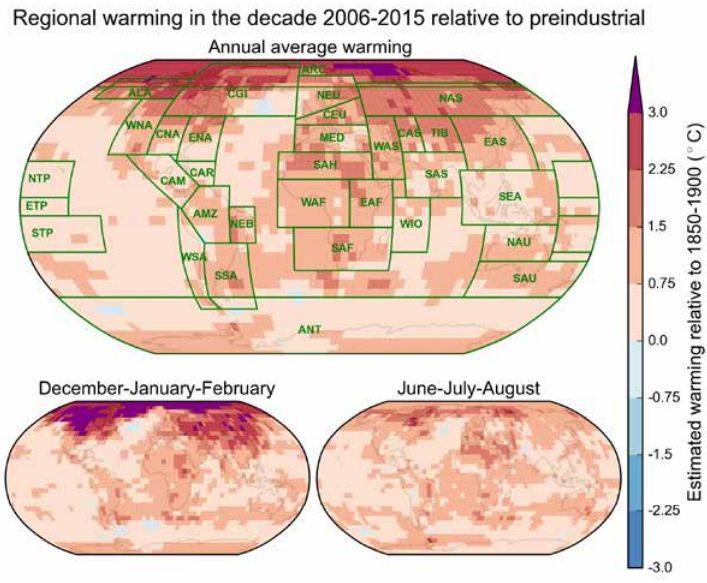
\includegraphics[scale=0.4]{Figura2}
    \caption{Calentamiento regional para la década de 2006-2015 relativa a 1850-1900 para una media anual.}
    \label{Figura 2}
\end{figure}


\subsection{Definición de las vías de $1.5$°C: Probabilidad, Transitoriedad, Estabilización, y Rebasamiento.}

Las vías consideradas en el reporte de la IPCC, consistentes con la literatura disponible en 1.5°C, primeramente enfocada en la escala de tiempo hasta 2100, reconociendo que la evolución del GMST después del 2100 es también muy importante. Dos grandes categorías de caminos de 1.5°C pueden ser usadas para caracterizar las opciones de mitigación e impactos: caminos donde el calentamiento se mantiene por debajo de 1.5°C en todo el siglo 21, y caminos en los cuales el calentamiento excede temporalmente el 1.5°C y regresa a ese mismo nivel, ambos antes y poco después del 2100. Los caminos no considerados son aquellos en los que el calentamiento rebasa los 1.5°C antes de llegar al 2100, pero deben regresar hasta el mismo nivel en algún siglo futuro.

\subsubsection{Vías donde se mantiene debajo de 1.5°C}

En esta categoría de caminos de 1.5°C, el calentamiento inducido por el humano aumenta monótonamente para estabilizarse en 1.5°C.

Si la reducción de emisiones no comienzan hasta que las temperaturas estén cerca del límite propuesto, los caminos donde se mantiene debajo de 1.5°C envuelven necesariamente la reducción mucho más rápida de emisiones de CO$_2$, combinado con reducciones rápidas en no-CO$_2$ y estos caminos también alcanzan los 1.5°C más temprano.

\subsubsection{Vías donde temporalmente de exceden los 1.5°C}

Con las vías en esta categoría, también referidas como vías \(overshoot\), GMST se eleva por encima de los 1.5°C alrededor o antes del 2100, subsecuentemente estabilizándose o continúa cayendo. Esto permite inicialmente reducción de emisiones más lentas o retrasadas, pero alentando GMST requiere emisiones netas negativas globales de CO$_2$.

En este reporte, las vías \textit{overshoot} son referidas como vías a 1.5°C, pero están calificadas por la cantidad de temperatura excedida, la cual puede ser un impacto sustancial en impactos de cambio climático irreversible.

\section{Impactos del $1.5$°C y más allá.}

\subsection{Definiciones.}

De acuerdo con el AR5 (Quinto Reporte de Evaluación), "impacto" en este reporte se refiere a los efectos del cambio climático en sistemas naturales y humanos. Los impactos pueden incluir efectos de peligro cambiante, como la frecuencia e intensidad de olas de calor. "Riesgo" se refiere a los impactos de potencial negativo de cambio climático donde algo de valor está en peligro, reconociendo la diversidad de valores. Los riesgos dependen de ciertas cosas como peligro, exposición, vulnerabilidad y posibilidad. Los riesgos de cambio climático pueden ser manejados a través de esfuerzos para mitigar los forzadores del cambio climático, adaptación de los sistemas impactados, y mediciones terapéuticas.


\subsection{Conductores de Impacto.}

Los impactos del cambio climático se dan por múltiples conductores de ambiente además de elevar las temperaturas, como elevar el CO$_2$ atmosférico, cambiando los patrones de lluvias, elevando los niveles oceánicos, aumentando la acidificación de los océanos, y eventos extremos como inundaciones, sequías, y olas de calor.

\section{Reflexión}

Es importante tener bien en cuenta que el mundo en el que vivimos está sufriendo en la mayoría por actividades humanas, este calentamiento que se ha generado ha sido comparado con la del total del calentamiento global. También debemos de tomar en cuenta que todavía estamos a tiempo de evitar una catástrofe mundial. Es necesario cambiar nuestros hábitos, para poder empezar a restaurar el mundo en el que vivimos. Ver que el cambio climático no es ningún invento y que es tan real que ya se han estado observando las consecuencias a partir de ignorar que nosotros contribuimos en gran parte al calentamiento de la temperatura media global.

% Referencias

\section{Referencias Bibliográficas}
\begin{itemize}
    \item Special Report: Global Warming of 1.5 ºC (2018). Consultado: 21 de Enero del 2019, de IPCC. Sitio Web: https://www.ipcc.ch/sr15/
    \item 8 Things You Need to Know About the IPCC 1.5°C Report: Consultado: 24 de Enero del 2019, de World Resources Institute. Sitio web: https://www.wri.org/blog/2018/10/8-things-you-need-know-about-ipcc-15-c-report
\end{itemize}
\end{document}